\documentclass[conference,letterpaper]{IEEEtran}
\usepackage[T1]{fontenc}
\usepackage[utf8]{inputenc}
\usepackage{cite}
\usepackage{amsmath,amssymb}
\usepackage{booktabs,tabularx}
\usepackage{placeins}
\usepackage{flushend}
\usepackage{pgfplots}
\pgfplotsset{compat=1.18}
\usepackage{xurl}
\usepackage[hidelinks]{hyperref}
\title{Beyond Polarity: Sentiment and Technical Purpose in Reddit Software-Update Discussions}
\author{\IEEEauthorblockN{Manu Mathew Jiss and Solomon Berhe}
\IEEEauthorblockA{School of Engineering and Computer Science\\
University of the Pacific, Stockton, California, USA\\
m\_jiss@u.pacific.edu, sberhe@pacific.edu}}
\begin{document}
\maketitle
\begin{abstract}
Emotional valence, a troubleshooting purpose, and an engineering action are different descriptions of a software-update discussion. We ask whether a lexicon score adds information to the same saved Reddit text when the decision is troubleshooting versus other update discussion. An earlier contrast between technical problem statements and general dissatisfaction is reproduced separately and is not the current label. On the Reddit-URL development posts, title-and-body sentiment does not reliably change a grouped text classifier. On the subset with a stored comment, adding sentiment features to the same full thread scores lower; that decrease is small, retrospective, and limited to a selected subset. A previously saved text-only model, not a sentiment model, scored lower on a later fresh test than on an earlier reserved test. Confirmed general-dissatisfaction posts do not reproduce the current mean valence gap. No human-confirmed resolution label is available. These findings belong to this snapshot and this lexicon.
\end{abstract}
\begin{IEEEkeywords}
software updates, Reddit, sentiment analysis, troubleshooting, negative results
\end{IEEEkeywords}

\section{Introduction}
Users write about crashes, changed behavior, and design disagreement after a software update. Those posts can share words such as ``update,'' ``broken,'' and ``fix'' while asking for different things. A negative tone does not establish that the writer is reporting a fault, and a troubleshooting label does not establish what an engineer should do next \cite{Chaparro2017Missing}, \cite{Bettenburg2008GoodReport}.

Software-engineering studies already warn that sentiment tools can disagree with one another and with human labels \cite{Jongeling2017Negative}, \cite{Lin2018HowFar}, \cite{Novielli2021Replication}. Domain lexicons reduce some of that mismatch \cite{Islam2018SentiStrengthSE}, but a polarity score is still not a purpose label. Reddit has been mined for requirements and release feedback \cite{Iqbal2021Reddit}, \cite{Singh2024ReleaseNotes}, and app-store studies document the cost of bad updates \cite{Hassan2020BadUpdates}. Those studies do not test whether sentiment, measured on the same saved text, changes a troubleshooting-versus-other-update decision.

An earlier analysis of 542 Reddit posts compared author and community valence under a different label pair: technical problem statement versus general dissatisfaction. That comparison motivated the sentiment question. It is not the current classification task. The current negative class is other update discussion. Only 68 Reddit-URL development posts are confirmed general-dissatisfaction discussions.

We ask four questions. \textbf{RQ1:} On the historical 542-post labels, do author and community valence still differ after the saved trajectories are recomputed, and which parts of that comparison depend on title-only author tracks? \textbf{RQ2:} On 2,050 Reddit-URL posts, does title-and-body sentiment improve a grouped text classifier of troubleshooting versus other update discussion? \textbf{RQ3:} On the subset with stored comments, does sentiment add information beyond the same full-thread text? \textbf{RQ4:} Does a mean valence gap remain when the negative class is restricted to confirmed general dissatisfaction?

The contribution is a bounded description of one lexicon on one saved collection. We separate historical and current labels, restrict the current evaluation to Reddit URLs, compare sentiment only against the same text, and keep the previously saved lower fresh-test score of the text-only model visible. We do not treat a null or lower development score as a universal property of sentiment analysis.

\section{Related Work}
Table~\ref{tab:prior} separates polarity research, negative-results research, and the nearest software-feedback studies. The distinction matters because a tool can be useful for one of those questions and uninformative for another.

\begin{table*}[t]
\caption{What prior studies estimate, and what this paper does not inherit.}
\label{tab:prior}
\centering
\footnotesize
\begin{tabularx}{\textwidth}{lXX}
\toprule
Study & Question they answer & Boundary for this paper \\
\midrule
Hutto and Gilbert \cite{Hutto2014VADER} & Rule-based polarity for short social-media text. & We use the published compound as a lexicon, not as a purpose model. \\
Islam and Zibran \cite{Islam2018SentiStrengthSE} & A software-engineering lexicon can score polarity more appropriately than a general lexicon. & Better polarity is not a troubleshooting decision. We do not swap in SentiStrength-SE. \\
Jongeling et al. \cite{Jongeling2017Negative} & The choice of sentiment tool can change the conclusion of a software-engineering study. & One lexicon cannot stand in for every tool. A null result here is local. \\
Lin et al. \cite{Lin2018HowFar} & Retraining a sentiment model on Stack Overflow text still produced negative results. & We do not retrain a sentiment model or claim that retraining would succeed. \\
Novielli et al. \cite{Novielli2021Replication} & Off-the-shelf software-engineering sentiment tools can disagree with each other and with raters. & Agreement with a purpose label is a further, separate question. \\
Iqbal et al. \cite{Iqbal2021Reddit} & Reddit threads can be mined as a requirements source. & Requirements categories are not our troubleshooting label. \\
Singh et al. \cite{Singh2024ReleaseNotes} & Reddit feedback can supplement release notes. & They do not test valence against a purpose classifier. \\
Hassan et al. \cite{Hassan2020BadUpdates} & Bad updates of free apps leave traces in store reviews. & Store ratings are not Reddit discussion purpose. \\
Ram{\'i}rez-Mora et al. \cite{RamirezMora2020Issues} & Issue and comment text can predict tracker-defined success. & We have no human-confirmed resolution label. \\
Huang et al. \cite{Huang2019Questions} & Questions raised during issue resolution are associated with delay. & Comment timing here is retrospective text, not a resolution process. \\
\bottomrule
\end{tabularx}
\end{table*}

Hutto and Gilbert designed VADER for short social-media text and published its rules and lexicon \cite{Hutto2014VADER}. Islam and Zibran built SentiStrength-SE because general-purpose scores misread software-engineering wording, including negation and technical terms that look negative in a general lexicon \cite{Islam2018SentiStrengthSE}. That is the mechanism behind our descriptive word check: an incident word can move a polarity score without establishing the writer's purpose. Lin et al. found that even a retrained model remained unreliable across software-engineering data sets \cite{Lin2018HowFar}. Jongeling et al. showed that substituting one sentiment tool for another can reverse a study's conclusion \cite{Jongeling2017Negative}. Novielli, Calefato, Lanubile, and Serebrenik extended the warning to software-engineering tools used off the shelf \cite{Novielli2021Replication}. We therefore report VADER as one prespecified lexicon. A different lexicon could move the estimates, and this paper does not measure that movement.

Comment text has been used for other decisions. Ram{\'i}rez-Mora et al. predicted whether tracker issues would succeed \cite{RamirezMora2020Issues}. Huang et al. studied questions raised while issues were being resolved \cite{Huang2019Questions}. Both outcomes were defined by tracker state or by the resolution record. Our saved posts have no comparable human-confirmed outcome, so a later comment is additional text. Iqbal et al. treated Reddit as a requirements source \cite{Iqbal2021Reddit}, and Singh et al. examined Reddit feedback as a supplement to release notes \cite{Singh2024ReleaseNotes}. Those are the closest source studies. Neither evaluates whether valence distinguishes troubleshooting from other update discussion.

\section{Collection and Labels}
The combined collection has 3,362 unique records: 542 historical posts and 2,820 later candidates. Development records for the current task are not all Reddit URLs. Of 2,080 development rows, 2,050 have \texttt{reddit.com} URLs and 30 are non-Reddit URL records: 28 troubleshooting and 2 other update discussion. Primary results use the 2,050 Reddit-URL rows. Table~\ref{tab:counts} lists every denominator used below. The 30 non-Reddit URL records are excluded from those primary results and appear only in the sensitivity and missingness checks.

\begin{table*}[t]
\caption{Sampling denominators. Protected tests are previously saved text-only scores and are not rescored here.}
\label{tab:counts}
\centering
\footnotesize
\begin{tabular}{lrrrl}
\toprule
Population & Rows & Positive & Negative & What the negative class is \\
\midrule
Historical corrected labels & 542 & 86 & 456 & Assigned dissatisfaction \\
Reddit-URL development & 2,050 & 1,658 & 392 & Other update discussion \\
\quad confirmed dissatisfaction & 68 & 0 & 68 & Inside the 392 \\
\quad other discussion types & 324 & 0 & 324 & Inside the 392 \\
Non-Reddit URL records & 30 & 28 & 2 & Excluded from primary results \\
Mixed-URL sensitivity & 2,080 & 1,686 & 394 & Reddit rows plus the 30 \\
Restricted type contrast & 1,726 & 1,658 & 68 & Not the current task \\
Stored-comment subset & 797 & 560 & 237 & Reddit rows with a comment \\
Reserved test, text only & 159 & 135 & 24 & Earlier text-only score \\
Fresh test, text only & 344 & 277 & 67 & Later text-only score \\
\bottomrule
\end{tabular}
\end{table*}

The historical corrected and assigned labels and the current task use different names. Historical positives are technical problem statements. Current positives are troubleshooting posts. Historical negatives are general dissatisfaction. Current negatives are other update discussion, a mixture of 324 posts with discussion type \texttt{other} and 68 posts with discussion type \texttt{general\_dissatisfaction}. Substituting one negative class for the other changes the question.

A constructed example, not a quotation, shows the difference. ``After the update, the browser stops opening pages'' is troubleshooting. ``The sync tool is now available as a one-click install'' is other update discussion and is not a dissatisfaction label. ``The new version is frustrating and releases are moving too fast'' can be confirmed general dissatisfaction while still sitting in the current negative class. The first and third can both receive a negative polarity score. Only the first is the current positive class. The second and third share the current negative class and do not share a dissatisfaction label.

Two protected tests were scored once, earlier, by a title-and-body text model. They are not sentiment scores, and this paper does not score them again. The reserved test has macro-F1 0.863. The fresh test, collected on identifiers outside the development set, has macro-F1 0.792. Fresh posts were not used to choose features or thresholds. The lower score is part of the text-only record.

Candidate posts were retrieved from \mbox{ReleaseTrain} \cite{ReleaseTrainDocs}. Its \texttt{/api/reddit/query/tps} and \texttt{/api/reddit/query/gds} endpoints supplied candidate pools, not confirmed labels. The historical raw responses were saved on 27~March~2026. The later candidate pages were saved on 5~October~2026. A post uses the October record when one was saved and the March record otherwise. Snapshots are not concatenated, and no post was refetched. We inspected \texttt{releasetrain-sentiment}~0.2.1 and did not use its scores. Its trajectory average is the mean of author comments, or zero when none is stored. This study's documented historical trajectory can use the title in that case. The valence scores in this paper come from this study's implementation. No field in the saved records is a human-confirmed statement that a comment resolved the reported problem. Absence of such a field is an unknown outcome.

\subsection{Comment missingness}
Saved comments are incomplete, and the incompleteness differs by class and source. Table~\ref{tab:miss} counts nonempty stored comments, author replies, and community comments. On Reddit, 1,098 of 1,658 troubleshooting posts (66\%) have no stored comment, compared with 155 of 392 other-update posts (40\%). All 30 non-Reddit URL records have no stored comment in this snapshot. The 797-post thread comparison is therefore a selected Reddit subset, not a description of every development row. On the 2,080-row development snapshot, stored comments are 38\% of the recorded comment counts. A comment timestamp is at or after the post in every stored comment we could compare, so comment features are retrospective.

\begin{table}[t]
\caption{Stored-comment coverage by source and current class. Counts are posts, not comments.}
\label{tab:miss}
\centering
\footnotesize
\setlength{\tabcolsep}{3pt}
\begin{tabular}{>{\raggedright\arraybackslash}p{2.15cm}rrrrr}
\toprule
Source and class & Posts & None & Author & Commun. & Both \\
\midrule
Reddit, troubleshooting & 1,658 & 1,098 & 362 & 554 & 356 \\
Reddit, other update & 392 & 155 & 112 & 235 & 110 \\
Non-Reddit URL records & 30 & 30 & 0 & 0 & 0 \\
\bottomrule
\end{tabular}
\end{table}

\section{Sentiment Definitions and Evaluation}
Three scores are defined before any model is fit, and they are not interchangeable.

\emph{Pre-discussion valence} is the VADER compound of the raw title, a newline, and the raw body \cite{Hutto2014VADER}. An empty or whitespace document scores 0, which collides with genuinely neutral text. Of the 2,050 Reddit-URL posts, 303 bodies are empty and 237 compounds are exact zeros. This score does not use comments.

\emph{Author-reply valence} is the mean compound of nonempty stored comments marked as the submitter or matching the author name. If no such comment exists, the descriptive mean is undefined. In the classifier, that case is represented by a zero together with a missingness flag. The title is never used as an author reply. That fallback was used in the historical trajectories and is one reason RQ1 is reported separately.

\emph{Community valence} is the mean compound of the other nonempty stored comments, with the same missingness rule. Author and community text are not given role tokens when they are concatenated into the thread document. API-precomputed sentiment, keyword features, and predicted categories are not used as inputs.

A keyword-first rule from the earlier study returns troubleshooting when a technical cue is present, unless the compound is strongly negative and no cue is present. That rule is a lexicon-and-keyword heuristic, not a pure sentiment model.

The text model is word and bigram TF--IDF, with minimum document frequency 2, at most 20,000 features, and sublinear term frequency, followed by class-balanced logistic regression ($C=4$, liblinear, seed 42). The vectorizer and any scaler are fit inside each training fold. The outer split is the saved five-fold grouped partition: near-duplicate posts, defined by a character five-gram Jaccard of at least 0.92 on the normalized title and body, stay together. Decision thresholds are chosen on three inner grouped folds of the training split only. The grid runs from 0.20 to 0.80 in steps of 0.05. The selected cutoff maximizes mean inner macro-F1, then mean inner F1 of the other-update class, then closeness to 0.5. Outer labels never choose the cutoff.

The paired quantity is macro-F1 of the sentiment-augmented model minus macro-F1 of the matched text model. Uncertainty uses 1,000 bootstrap resamples of posts and, separately, 1,000 resamples of duplicate groups, both with seed 42. Naive Bayes and a linear SVM are continuity checks on title-and-body text only. Naive Bayes is not class-balanced and its threshold is selected on the same inner grid. The SVM uses its default decision margin rather than that grid.

Two comparisons must stay distinct. The pre-discussion comparison uses title and body only, on all 2,050 posts. The thread comparison uses one fixed document: title, body, and stored comments in time order, with the same string in the text model and in the text half of the hybrid. The hybrid adds five columns: the pre-discussion compound, the author-reply mean or zero, the community mean or zero, and the two missingness flags. The first three columns are standardized on the training fold. A different contrast, title-and-body text versus title-and-body text plus comment-derived sentiment, gives the hybrid access to comments the baseline never sees. That contrast is not evidence about sentiment beyond comment text, and we do not use it as a result.

\section{Results}
\subsection{Historical 542 posts}
Recomputing the saved trajectories mismatches none of the stored metric rows. Stored comments cover 10,416 of 17,549 recorded comments on the labeled posts (59\%), and 396 posts are short of the recorded count. Author tracks are title-only for 205 posts, 24 technical and 181 general-dissatisfaction. On the full file, author means are $0.009$ versus $0.191$ (Welch $p=4.7\times10^{-5}$) and absolute author--community divergence is $0.371$ versus $0.287$ (Mann--Whitney $p=0.009$). Community means are $0.168$ versus $0.194$ (Welch $p=0.33$).

Removing the 205 title-only tracks leaves 62 technical and 275 general-dissatisfaction posts. Author means remain lower for technical posts, $0.077$ versus $0.261$ (Welch $p=8.2\times10^{-4}$). Absolute divergence does not: $0.373$ versus $0.302$, Mann--Whitney $p=0.060$. The full-file divergence result therefore depends on a construction that treats titles as author replies. Author slope and author early-versus-late contrasts are not significant on the full file (Welch $p=0.27$ and $p=0.43$). Community slope is $p=0.083$ by Welch's test and $p=0.026$ by a Mann--Whitney test, so the two tests disagree and we do not claim a community change over the thread. These statements describe the historical corrected labels only. Figure~\ref{fig:valence}(b) shows the full-file author and community means. It includes the 205 title-only author tracks, so the author bars are not estimates from author replies alone.

\subsection{Current Reddit-URL task}
Table~\ref{tab:pre} reports grouped out-of-fold scores on all 2,050 posts. Title-and-body text reaches macro-F1 0.832. VADER alone reaches 0.534, near the majority baseline of 0.447. Text plus the title-body compound reaches 0.833. The difference is $+0.001$. The post-level 95\% interval is $-0.012$ to $+0.015$, and the duplicate-group interval is $-0.013$ to $+0.015$. Both include zero. Other-update F1 changes by $+0.001$, with an interval from $-0.020$ to $+0.023$ that also includes zero. In this development snapshot, the lexicon does not reliably add information to the same title and body. The same text specification scored 0.863 on the reserved test and 0.792 on the fresh test in the earlier, unchanged evaluations. Those two numbers are text-only. The fresh confusion matrix has 46 of 67 other-update posts and 252 of 277 troubleshooting posts correct.

Mean title-body compound is $-0.064$ for troubleshooting and $+0.194$ for other update discussion. Splitting that negative class by assigned discussion type, the 324 posts typed \texttt{other} have mean $+0.249$ and the 68 dissatisfaction posts have mean $-0.068$. Figure~\ref{fig:valence}(a) shows those three types on the Reddit-URL posts only. The positive side of the current gap is the \texttt{other} type, not confirmed dissatisfaction.

\begin{figure*}[t]
\centering
\begin{minipage}{0.48\textwidth}
\centering
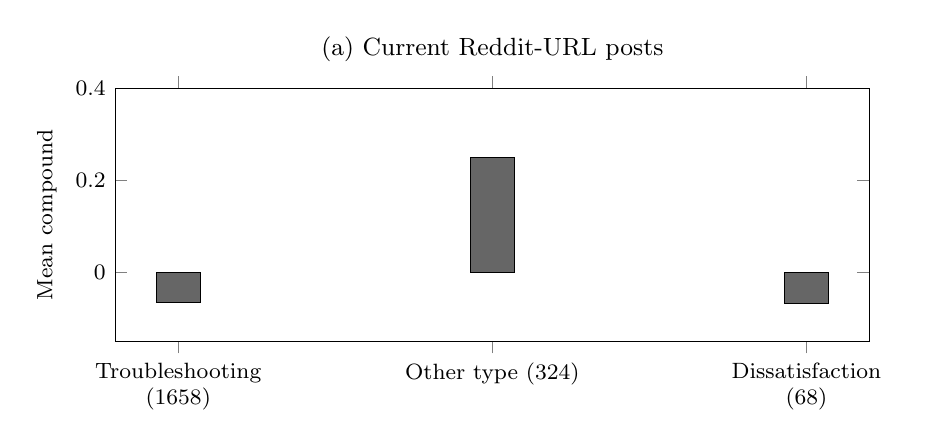
\begin{tikzpicture}
\begin{axis}[
    ybar,
    bar width=16pt,
    width=0.92\linewidth,
    height=4.8cm,
    ymin=-0.15, ymax=0.40,
    ylabel={Mean compound},
    symbolic x coords={tt, ot, gd},
    xtick=data,
    xticklabels={Troubleshooting (1658), Other type (324), Dissatisfaction (68)},
    x tick label style={font=\footnotesize, align=center, text width=2.3cm},
    y tick label style={font=\footnotesize},
    ylabel style={font=\footnotesize},
    title={(a) Current Reddit-URL posts},
    title style={font=\small},
    axis line style={thin},
    tick style={thin},
]
\addplot[fill=black!60] coordinates {(tt,-0.0644) (ot,0.2491) (gd,-0.0680)};
\end{axis}
\end{tikzpicture}
\end{minipage}\hfill
\begin{minipage}{0.48\textwidth}
\centering
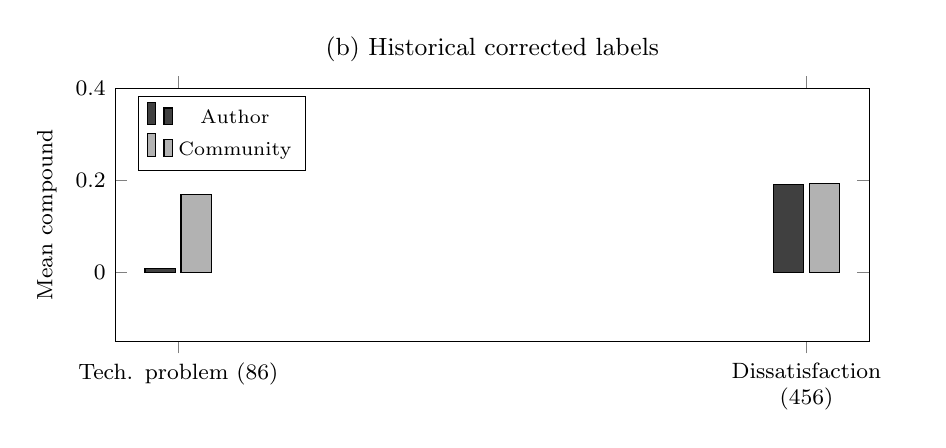
\begin{tikzpicture}
\begin{axis}[
    ybar,
    bar width=11pt,
    width=0.92\linewidth,
    height=4.8cm,
    ymin=-0.15, ymax=0.40,
    ylabel={Mean compound},
    symbolic x coords={tps, gds},
    xtick=data,
    xticklabels={Tech. problem (86), Dissatisfaction (456)},
    x tick label style={font=\footnotesize, align=center, text width=2.6cm},
    y tick label style={font=\footnotesize},
    ylabel style={font=\footnotesize},
    title={(b) Historical corrected labels},
    title style={font=\small},
    legend style={font=\scriptsize, at={(0.03,0.97)}, anchor=north west},
    axis line style={thin},
    tick style={thin},
]
\addplot[fill=black!75] coordinates {(tps,0.0091) (gds,0.1911)};
\addplot[fill=black!30] coordinates {(tps,0.1683) (gds,0.1940)};
\legend{Author, Community}
\end{axis}
\end{tikzpicture}
\end{minipage}
\caption{Mean VADER compound under two label systems that are not interchangeable. Panel (a) is the title-and-body score on 2,050 Reddit-URL posts, split by assigned discussion type. Panel (b) is the saved full-file trajectory on 542 posts with historical corrected labels; its author means include 205 title-only tracks. The vertical scales match so the magnitudes can be compared, but the panels are not the same contrast and neither is a causal effect. The current positive class in panel (a) is troubleshooting, which is not the historical technical-problem label in panel (b).}
\label{fig:valence}
\end{figure*}

On the same folds, class-balanced SVM text classification reaches 0.820 and the keyword-first heuristic reaches 0.685. Unbalanced Naive Bayes reaches 0.551 and predicts troubleshooting for almost every post. The logistic-regression text model remains the continuity baseline. A sensitivity fit on all 2,080 development rows gives text 0.835 and text plus compound 0.836. The difference is $+0.001$ and its interval includes zero. Adding the 30 non-Reddit rows does not change the conclusion.

\begin{table}[t]
\caption{Pre-discussion scores on 2,050 Reddit-URL posts. Macro-F1 uses inner-fold thresholds.}
\label{tab:pre}
\centering
\begin{tabular}{lc}
\toprule
Model & Macro-F1 \\
\midrule
Majority class & 0.447 \\
VADER compound only & 0.534 \\
Keyword-first heuristic & 0.685 \\
TF--IDF logistic regression & 0.832 \\
Same text plus VADER compound & 0.833 \\
\bottomrule
\end{tabular}
\end{table}

\subsection{Stored-comment subset}
The 797 posts with a stored comment are 560 troubleshooting and 237 other update discussion. Full-thread text reaches macro-F1 0.866. The same text plus the prespecified sentiment columns reaches 0.839. The difference is $-0.027$. The post-level interval is $-0.049$ to $-0.004$, and the group-level interval is $-0.051$ to $-0.005$. Both exclude zero in this subset. That is a lower score on this comparison, not evidence that sentiment features are generally harmful. Only 14 of the 797 posts share a duplicate group, so the group interval mostly repeats the post interval. Both-role coverage is 466 of 2,050 Reddit-URL posts (23\%), below a predeclared 50\% bar for a strong comment claim. The result does not say that sentiment changes a future decision, and it does not say that a comment fixed an issue.

VADER on title and body alone scores 0.535 on this subset. The keyword-first heuristic scores 0.761. Neither replaces the thread text. Table~\ref{tab:thread} shows that the lower score appears in both classes: other-update F1 falls from 0.812 to 0.775, and troubleshooting F1 falls from 0.919 to 0.903.

\begin{table}[t]
\caption{Matched full-thread comparison on 797 posts with a stored comment.}
\label{tab:thread}
\centering
\footnotesize
\begin{tabular}{lccc}
\toprule
Model & Macro-F1 & Other F1 & Trouble F1 \\
\midrule
Full-thread text & 0.866 & 0.812 & 0.919 \\
Same text plus sentiment & 0.839 & 0.775 & 0.903 \\
\bottomrule
\end{tabular}
\end{table}

\subsection{Confirmed dissatisfaction}
On the 1,726 Reddit-URL posts labeled either technical troubleshooting or general dissatisfaction, mean title-body compound is $-0.064$ versus $-0.068$. The difference is $+0.004$ and its interval includes zero. Author-reply and community means on the observed comments also have intervals that include zero; only 15 of the 68 dissatisfaction posts have a stored author reply. Text classification of this restricted pair reaches macro-F1 0.658, and adding the title-body compound changes it by $+0.010$ with an interval that includes zero. VADER alone predicts the troubleshooting class for every post. The valence gap in the current task is a gap against other update discussion, not a gap against confirmed general dissatisfaction.

\subsection{Technical words and evaluative wording}
We counted two closed word lists on the title and body of the 2,050 Reddit-URL posts. The incident list is the earlier title mask without ``update'' and ``upgrade,'' because the collection is already update-scoped: error, bug, fix, crash, install, broken, issue, problem, dependency, and config, with obvious variants. The discontent list is evaluative rather than incident-like: hate, annoying, frustrating, disappointed, useless, terrible, awful, worst, stupid, garbage, trash, ridiculous, sucks, and horrible, again with obvious variants. The lists were fixed before the counts were read. This is a description of co-occurrence. It is not a masking experiment, and it does not estimate the causal effect of any word.

Table~\ref{tab:words} shows the cells. An incident term appears in 1,258 of 1,658 troubleshooting posts (76\%) and in 154 of 392 other-update posts (39\%). A discontent term appears in 167 troubleshooting posts (10\%) and 43 other-update posts (11\%). Within incident-only posts, the mean compound is $-0.060$ for troubleshooting and $+0.355$ for other update discussion. Discontent-only posts are negative in both classes, but there are only 33 and 13 of them. The class difference in polarity is therefore not the same thing as a difference in evaluative discontent, and the presence of an incident word does not by itself determine the sign of the score.

The following illustrations are constructed to show the cells. They are not quotations, and they are not identifiers. A troubleshooting post can say that a security update left an application reporting an error; a lexicon can score ``error'' as negative even when the sentence is a request for help. An other-update post can announce that a feature is now a one-click install; ``install'' is technical, and the sentence can still be positive. A dissatisfaction post can say that a new version is frustrating and that releases are moving too fast, with little incident vocabulary. A troubleshooting post can say that a browser no longer opens pages after an update and match neither list. Frequency differences describe the saved text. They do not show that removing a word would change the label or the classifier.

\begin{table}[t]
\caption{Descriptive title-and-body cells on 2,050 Reddit-URL posts. Parentheses are mean VADER compound. No causal effect is estimated.}
\label{tab:words}
\centering
\footnotesize
\begin{tabular}{lrr}
\toprule
Cell & Troubleshooting & Other update \\
\midrule
Incident term only & 1,124 ($-0.060$) & 124 ($+0.355$) \\
Discontent term only & 33 ($-0.275$) & 13 ($-0.223$) \\
Both lists & 134 ($-0.228$) & 30 ($+0.056$) \\
Neither list & 367 ($+0.002$) & 225 ($+0.148$) \\
\bottomrule
\end{tabular}
\end{table}

\subsection{What purpose still leaves open}
A separate diagnostic review of 237 reconfirmed troubleshooting posts, drawn from the Reddit development pool, found a specific symptom in every reviewed post, reproduction context in 108, and error evidence in 40. In 30 intact cases, two engineers sometimes cited similar facts and chose different first actions. Those observations are supporting context. They are not sentiment results. They bound what a purpose label can mean: it can sort discussion, and it cannot show that a comment resolved the report or that a reviewer should take a particular next step.

\section{Discussion}
The current valence gap and the historical valence gap answer different questions. Other update discussion is more positive on average than troubleshooting. Confirmed general dissatisfaction is not. A sentiment feature can look informative when the negative class contains announcements, advice, and mixed reactions, and uninformative when both classes are complaint-like. That is a statement about these labels, not evidence that sentiment detects dissatisfaction in general.

The thread result should be read at the size we measured. A macro-F1 drop of $0.027$, with an upper interval endpoint near $-0.005$, says the added columns did not help this selected snapshot. It does not say that sentiment features harm classification outside that snapshot. The pre-discussion interval, which uses every Reddit-URL post and the same text in both models, includes zero. Together the two comparisons do not support a claim that this VADER feature improves the decision here. They also do not license a claim about all sentiment tools or all software-update communities.

The text-only fresh test is the right place to see that the text model itself moves. The same specification and threshold scored 0.863 on 159 reserved posts and 0.792 on 344 fresh posts. We did not retrain on the fresh identifiers, and we did not attach sentiment features to that test. A development score of 0.832 would overstate how stable the text model is.

\section{Threats to Validity}
The current negative class mixes discussion types. A valence difference against that mixture can disappear under the historical dissatisfaction definition, as it does here. Comment rows are missing for most troubleshooting posts and for every non-Reddit URL record in this snapshot, so the 797-post model is a selected-subset description. Duplicate grouping matters in the design, but this subset contains little duplication. VADER's zero for empty text confounds neutral sentiment with missing body text. The word lists are closed and incomplete; posts can express a fault or a complaint without matching them. Counts of those lists are not a mediation analysis. Thresholds and vectorizers were fit without the protected tests, but the development comparisons are still development comparisons. No causal effect of sentiment, comments, wording, or diagnostic fields is identified.

\section{Conclusion}
On this saved collection, emotional valence, troubleshooting purpose, and engineering action come apart. Reproducing the historical trajectories confirms an author-valence difference under the old labels and does not confirm a community difference or a change over the comment sequence. On the current Reddit-URL task, title-and-body sentiment does not reliably improve a grouped text classifier. Adding sentiment features to the same full thread scores lower in the comment subset, under the limits above. The lower fresh-test score of the text-only model remains 0.792. Confirmed general dissatisfaction does not reproduce the current mean valence gap. The practical implication is local: the post text can help organize troubleshooting discussion in this setting, and a sentiment score from this lexicon is not evidence of purpose, resolution, or the next engineering action.

\section*{Data Availability}
The public project repository is {\renewcommand\UrlBreaks{\do\/}\url{https://github.com/SE4CPS/Research-on-Software-Updates}}. Development identifiers, corrected labels, and the scripts for these comparisons are archived with the study. Protected tests were not used to select features or thresholds and were not rescored for this paper.

\bibliographystyle{IEEEtran}
\bibliography{references}
\end{document}
